\subsection{Topic Model}

5000 iterations of randomized search were performed to find the optimal parameters for the topic model. The highest score was $0.3867$ and the lowest was $0.1975$. 6 of the 5000 models had a coherence score higher than $0.38$.

Two models are presented for good measure. The highest coherence score was $0.3867$, followed by a score of $0.3842$. The parameters of the corresponding topic models are listed in table 5 as well as other data. An interactive visualization of both models using pyLDAvis is available in the appendix.

\begin{table}[!h]
    \centering
    \begin{tabular}[\textwidth]{lcccccc}
        \hline
        \textbf{Model}  & No. Topics & $\alpha$ & $\beta$ & min\_df & max\_df & $C_v$ \\ \hline
        Model 1 & 2 & 0.05 & 0.02 & 0.07 & 0.30 & 0.3867 \\
        Model 2 & 6 & 0.07 & 0.05 & 0.02 & 0.20 & 0.3842 \\ \hline
    \end{tabular}
    \caption{Parameters of the topic models.}
\end{table}

\begin{figure}[H]
    \centering
    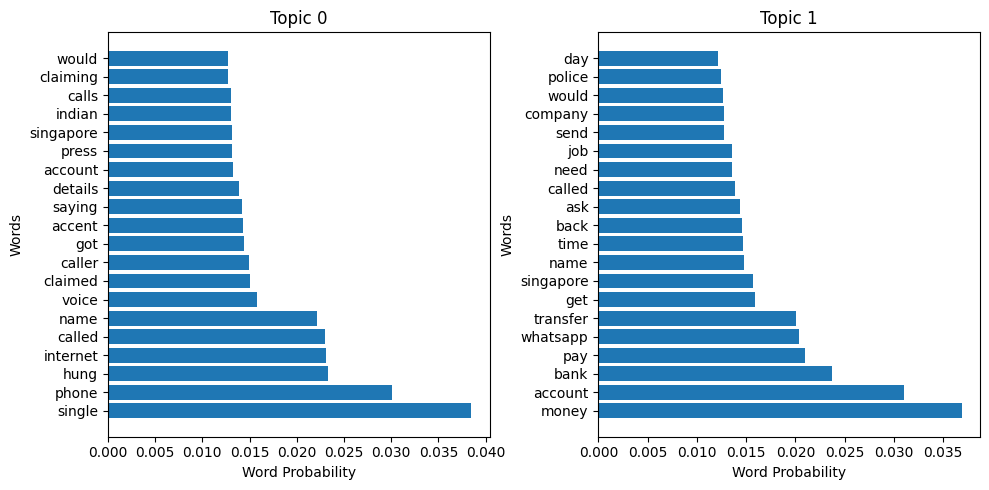
\includegraphics[width=\textwidth]{resources/model_n_2.png}
    \caption{Visualization of the topics in model 1.}
    \label{fig:topic_model_1}
\end{figure}

Figure 6 shows a visualization of the topics of model 1 and the distribution of the top 20 most common words in them.

Topic 0 was present in 55.7\% of all documents, while topic 1 was present in 60.2\%. Using gensim's implementation of the Hellinger Distance, a metric to measure the similarity between two probability distributions, the distance between the two topics was $0.45$.

\begin{figure}[H]
    \centering
    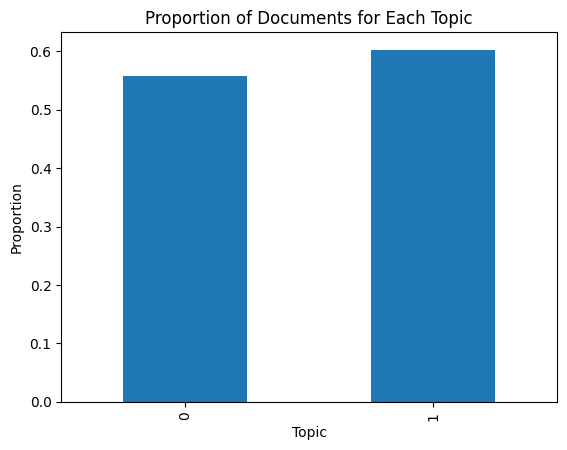
\includegraphics[width=0.5\textwidth]{resources/proportion_n_2.png}
    \caption{Proportion of model 1 topics in the corpus.}
    \label{fig:proportion_n_2}
\end{figure}

Model 2, which contains 6 topics, is visualized similarily below in figures 8 and 9. The most prominent topic in the corpus is topic 0, which is present in 35.7\% of all documents, followed by topic 5 at 32.8\%, topic 2 at 32.1\%, topic 4 at 31.3\%, topic 3 at 25.2\% and topic 1 at 23.0\%.

\begin{figure}[H]
    \centering
    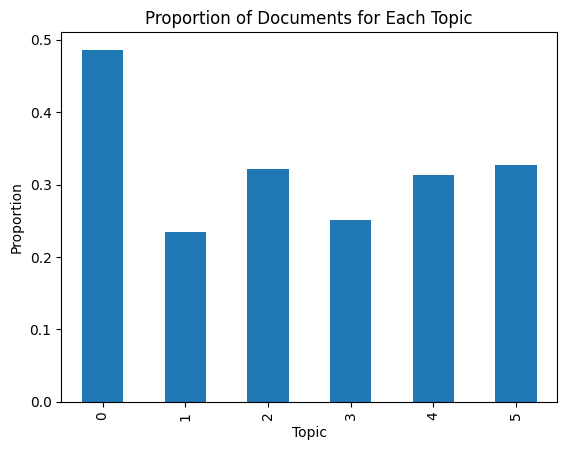
\includegraphics[width=0.5\textwidth]{resources/proportion_n_6.png}
    \caption{Proportion of model 2 topics in the corpus.}
    \label{fig:proportion_n_6}
\end{figure}

Since the number of topics is higher than 2, the Hellinger Distance is presented as a matrix that shows the distance between each pair of topics. The matrix is shown in table 6.

\begin{table}[H]
    \centering
    \resizebox{\textwidth}{!}{
      \begin{tabular}{|*{7}{>{\centering\arraybackslash}m{1.8cm}|}}
            \hline
            Topic & 0 & 1 & 2 & 3 & 4 & 5 \\
            \hline
            0 & 0.000 & 0.503 & 0.498 & 0.463 & 0.533 & 0.439 \\
            \hline
            1 & 0.503 & 0.000 & 0.430 & 0.448 & 0.421 & 0.446 \\
            \hline
            2 & 0.498 & 0.430 & 0.000 & 0.405 & 0.386 & 0.388 \\
            \hline
            3 & 0.463 & 0.448 & 0.405 & 0.000 & 0.425 & 0.429 \\
            \hline
            4 & 0.533 & 0.421 & 0.386 & 0.425 & 0.000 & 0.437 \\
            \hline
            5 & 0.439 & 0.446 & 0.388 & 0.429 & 0.437 & 0.000 \\
            \hline
        \end{tabular}
      }
    \caption{Hellinger Distance matrix of model 2.}
    \label{tab:hellinger_distance_matrix}
  \end{table}

\begin{figure}[H]
    \centering
    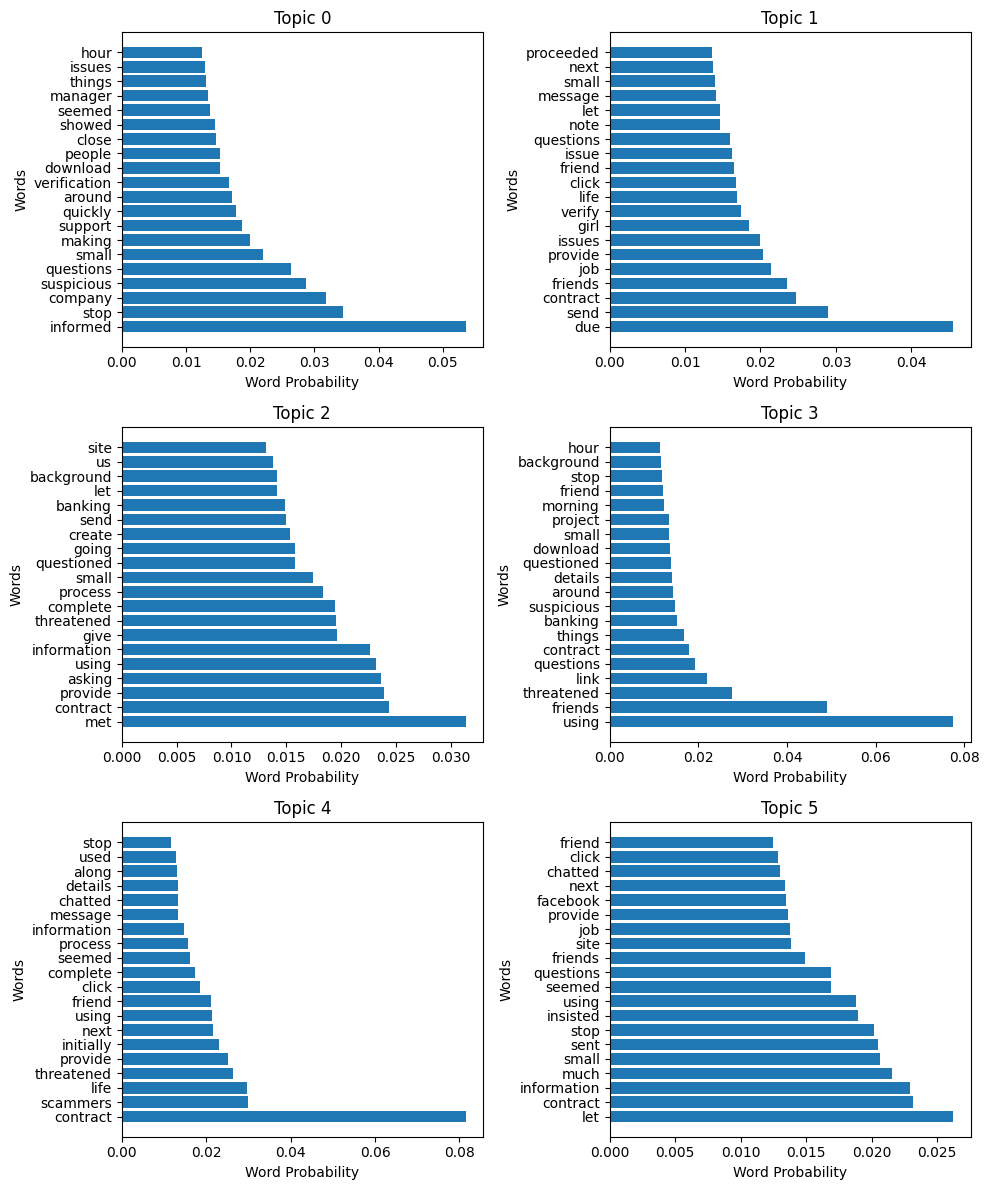
\includegraphics[width=\textwidth, height=\textwidth]{resources/model_n_6.png}
    \caption{Visualization of the topics in model 2.}
    \label{fig:topic_model_2}
\end{figure}

